\documentclass{ltjsarticle}
\usepackage{docmute} 
\usepackage{myStyle} 


\begin{document}

\chapter{Parameter Estimation using Bayesian Method}
\label{chapter25}
As a third method for estimating the parameters, we consider estimation using Bayesian methods. The advantage of Bayesian methods is that they allow for the likelihood function to be transformed into a probability distribution function, and the certainty of the estimated value can be expressed in terms of probability. We also consider how these estimation methods are used in statistical inference and actual statistical models. The development of probabilistic programming languages has simplified these calculations, and we mention the method of approximating probability distributions using random numbers (MCMC methods).
\section{Reconsidering Bayes' Theorem}
Last time we explained estimation using the maximum likelihood method, and finally talked about Bayes' theorem as an introduction to the Bayes method. Here, we would like to review these relationships and take another look at them.

\subsection{Prior Distribution}
I would like to start by explaining the prior distribution first.

The prior distribution is a distribution given in advance for the probability parameter. Some people may think it's strange to know something beforehand about how the parameters will turn out.

Each term in Bayes' equation is expressed in terms of probability. Regarding the numbers known as probability, please refer back to chapter 6 for a reminder, but there are three conditions involved.
\begin{enumerate}
	\item 確率の値は非負
	\item 全標本空間におけるすべての事象の確率の合計が1.0
	\item 任意の2つの相互に排他的な事象について，どちらか一方が発生する確率は個々の確率の和
\end{enumerate}

So it was said. And if this condition is met, then anything can be thought of as probability and calculated accordingly.

The probability learned in high school math, for most of you, was something like "count all possible outcomes and express the ratio." This is called \keytermE{frequentist} probability, which considers probability as the limit of an infinitely extended sequence. On the other hand, even for numbers that represent the strength of belief, such as the probability of precipitation, it is considered probability if it satisfies the above conditions. Let's call this concept of probability \keytermE{subjective probability} or \keytermE{Bayesian} probability. 

Note that there is a historical context in these terms. Frequentist probability was initially developed, and then the Bayesian concept of probability was introduced. Neither is right or wrong, it is just a matter of thinking. The academia is concerned with correctness, not with specific values or advocacy. Therefore, a neutral position that can be used for both is the probability created by three axioms. There used to be a controversy between frequentist vs. Bayesian (not about correctness), but now there is an effort to eliminate the expression of "…ism" probability because it is too dogmatic and represents the past opposition of frequentist vs. Bayesian. However, this might be too principled and merely semantic. If you are interested in the history of ideological conflict, there is an interesting book for you to read \citep{mcgrayne2011theory}. For now, let's stick to these terms because they are easy to understand.


\section{Concept of Probability and Statistical Inference}


I don't want to decide superiority or inferiority based on conflicting principles or beliefs, but it's a fact that the way to think about the parameters differs between frequentist thinking and Bayesian thinking. With frequentist thinking, if you repeat an infinite number of trials, you should eventually arrive at the answer, in other words, "the truth is always one." However, since it's not directly understandable, you can only gradually approach it. As shown in the top row of Figure \ref{fig::25_06}, you can express confidence intervals with each trial, but you will continue the decision between 0/1 for whether it crosses the true value (in the figure, 0.5 is used as the true value).

Estimation using Bayesian methods based on subjective probability takes into account the fact that the parameter value is originally unknown, and expresses this by the use of probability. Initially, a broad probability distribution is considered over the entire range. Through the accumulation of data from each trial, this distribution becomes narrower and the certainty that the true value is in a particular range is increased.
\begin{figure}[ht]
   \centering
   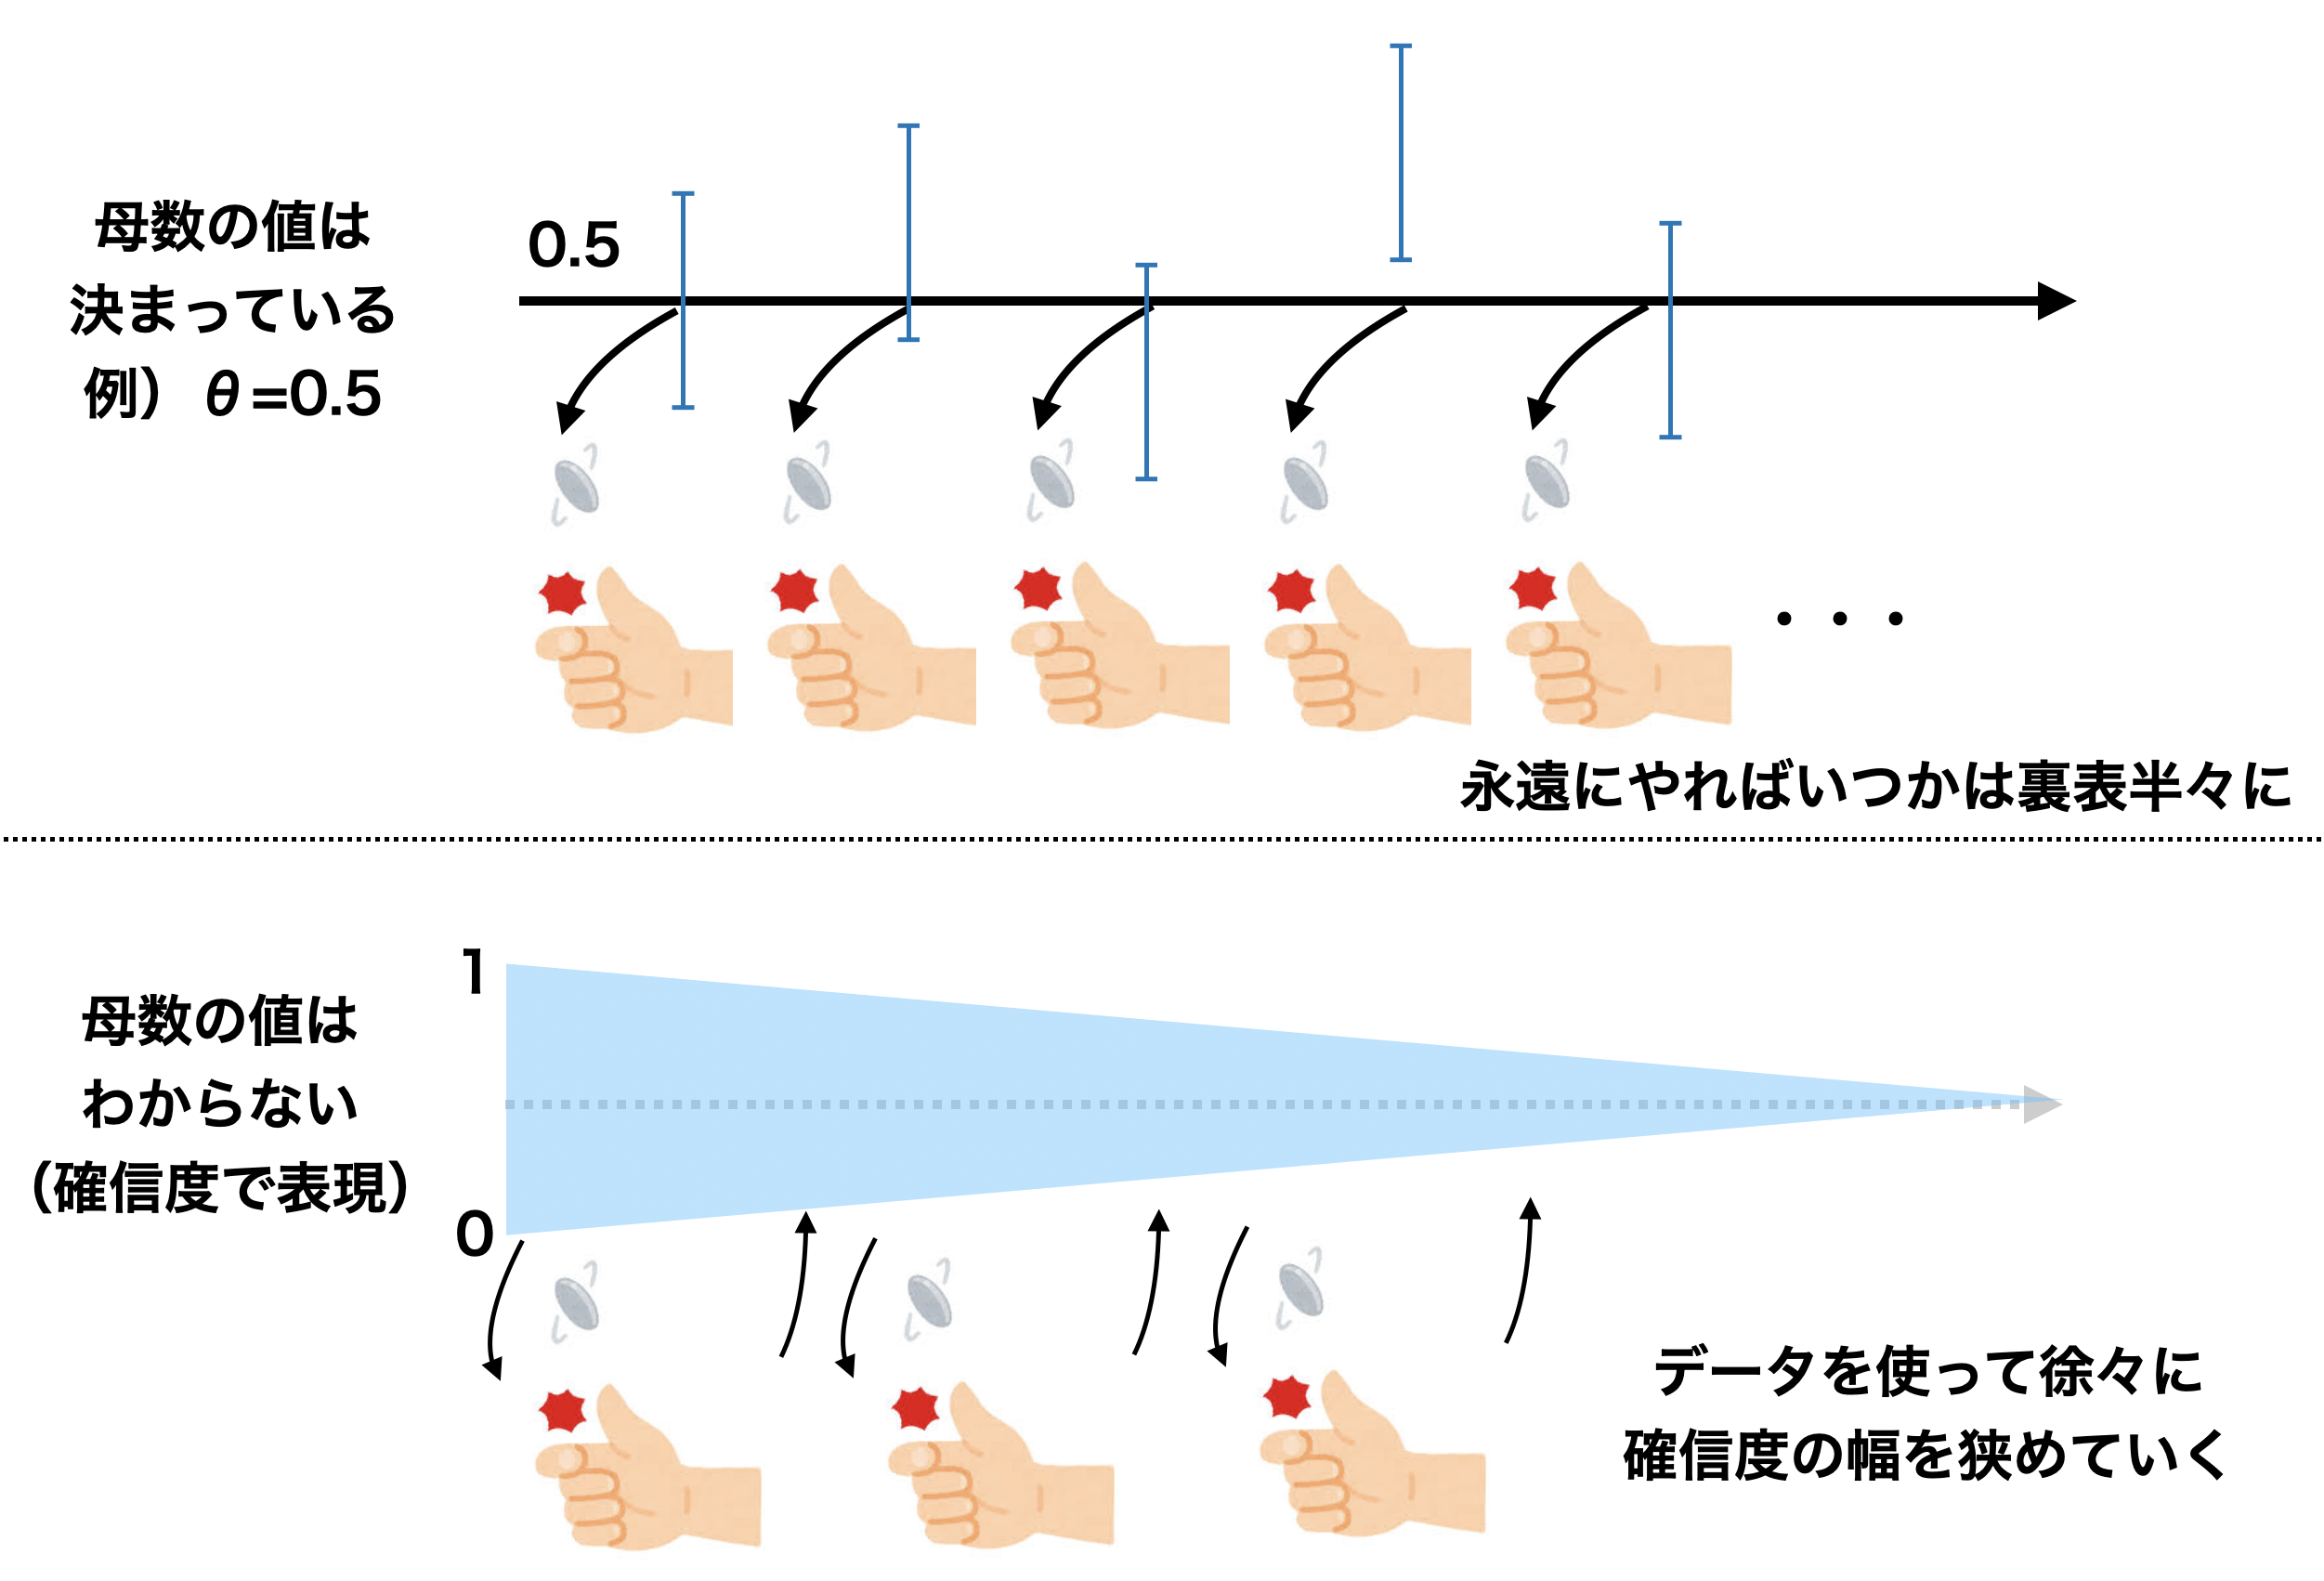
\includegraphics[keepaspectratio,width=0.8\linewidth]{../images/text25/slide25_06.png}
   \caption{Two concepts about probability}
   \label{fig::25_06}
\end{figure}

There is no definitive answer as to whether it can be thought that the true value is determined as a single constant when making estimations using Bayes' theorem. It is possible to regard the parameters as being determined by a constant, but with only a probabilistic understanding, or to consider that the parameters are fundamentally probabilistically distributed. Either interpretation is acceptable\footnote{There are similarities between these different interpretations and the philosophical differences between Bohr and Einstein's interpretation of quantum mechanics. Einstein famously stated that "God does not play dice", meaning that he believed in the certainty of physical phenomenon. On the other hand, the Copenhagen interpretation, led by Bohr, asserted that physical phenomenon ultimately exist in a probabilistic state, as exemplified by Schrödinger's cat existing in a superposition of both being alive and dead (and unknown until observed). While quantum mechanics has prevailed as the dominant theory in modern physics, it is understandable to sympathize with Einstein's perspective.}.

In modern times, or as a user of statistics, it may be pragmatic to take the approach that "what is practical is the correct way of thinking". Alternatively, in the applied field called information statistics, where the focus is not on the estimated values of parameters, there is a way of thinking that emphasizes the uncertainty of prediction by the model rather than the uncertainty of the estimate itself, assuming a "world of true distribution" beyond the population. In any case, I hope you pay attention to the differences in meaning represented by these methods.
\section{Approximation Algorithms Using Randomization}
Estimation using Bayes' theorem has quickly spread in the past decade. Although Reverend Thomas Bayes formulated Bayes' theorem in the 18th century, it wasn't fully utilized until the 21st century. One reason may be that Bayes believed the concept of inverse probability, which involves searching for fundamental reasons behind observed data, may go against the will of God. As a result, he was hesitant to publish his work. Additionally, Fisher, who created analysis of variance, was against the Bayesian approach and oppressed it. Bayesian statistics was also used for military purposes such as code-breaking, which prevented results from being published. However, a more positive reason for the delay may be that it was difficult to calculate practically until recent computer technology advancements allowed for the development of useful calculation methods, specifically the technical breakthrough of a process called "Markov Chain Monte Carlo."

The practical difficulty in Bayesian statistics is that as the model becomes more complex, the "calculation combining multiple probability functions" becomes so complex that it is impossible to handle. Before MCMC was developed, the method involved finding a probability distribution that could be calculated by finding a good combination and targeting the area where the peak is likely to be around this area, or dividing the interval into fine meshes and calculating it anyway. However, it was still very difficult.

MCMC (Markov Chain Monte Carlo) is one method of searching for approximate answers. The name MCMC is made up of two parts: "Markov chain" and "Monte Carlo method". Markov chain is a method of creating transition rules that lead to the desired probability distribution state, and Monte Carlo method is an algorithm that generates random numbers. By combining these two methods, it is possible to create a random number generator that can obtain samples even when the shape of the probability distribution is unknown.

The goal of Bayesian statistics is to create a posterior distribution. In simple cases, such as setting the prior distribution to a uniform distribution and using a Bernoulli distribution for likelihood, there are no particular problems. However, when there are parameters for a certain probability distribution, and a probability distribution that generates them, such as a hierarchically nested model, there is a situation where "the shape of the final posterior distribution is unknown". While the characteristics of probability distributions with names such as normal distributions and Poisson distributions can be clearly understood, those made by combining them become composite functions without names, and it is sometimes impossible to imagine what shape they take. Using Markov chains is a mathematical technique that can create the shape of such composite functions.

The Monte Carlo method is a technique for generating random numbers. Random numbers are those without any regularity, but it is quite difficult to create them. When humans write down numbers randomly within the range of 0 to 9, unintentionally an uneven pattern is created\footnote{There is a slogan "lie of 538", which says that when humans try to randomly generate numbers, the numbers 5, 3, and 8 tend to appear more frequently. It is said to be true but we cannot confirm its reliability as there is no evidence.}. You may think that computers (such as R) have random numbers, but computers are always rational machines. Although it appears to be working with random numbers, the algorithm to generate numbers that look like random numbers is embedded in the computer, so it is only pseudo-random. The random numbers created by computers, of course, have less regularity than those generated randomly by humans, but fundamentally, they are still pseudo-random.
\begin{itemize}
   \item Update the internal state $S_t$ using some function $g$; $S_{t+1}=g(S_t)$
   \item Generate real-valued outputs using some function $h$ applied to the internal state $S_t$; $x = h(S_t)$
\end{itemize}

This is generated by iteratively repeating the step ($t=1,2,3\ldots$). Once such a random sequence is created, it is easy to fit it to the shape of a normal distribution or a binomial distribution to output it. There is a probability distribution-based random number generation technique known as Markov Chain Monte Carlo (MCMC) that is based on this step-by-step calculation method. By the way, with smartphone apps and so on, "gacha pulling" is also based on random number generation inside and only pseudo-random numbers are generated to "make it look like a coincidence". When I play games, I lose my motivation if I think of the pseudo-random numbers and that "I am being played by someone somewhere", so I am not interested in scenes like gacha pulling. As expected, in multiplayer games, unexpected behavior is more interesting when humans are behind it, and I think it is fun to enjoy real randomness that is not pseudo in the real world than in games. What do you think?

The MCMC (Markov Chain Monte Carlo) method is a technique that allows the generation of random samples of any probability distribution, regardless of its shape. Even if the shape and function of the posterior distribution are unknown, random samples can be generated through this technique. With the huge advancements in computer technology today, large numbers of random samples can be generated in an instant.

Now, as you may have felt while executing probability distributions in R, if you generate a large number of random numbers and draw their histogram, it gradually approaches the shape of the probability distribution function. Even if you don't know the specific probability distribution function, if you draw the histogram and look at its outline, you can see the shape of the probability distribution function. Figure 25.07 shows an example of generating normal random numbers in R. When there are only 100 random numbers (top left of the figure), the histogram looks jagged, but when there are 1000 (top right) there seems to be a pattern, and with 10,000 (bottom left), there are some distorted areas, but it is generally symmetrical with a bell-shaped curve, and with 100,000, it almost becomes a theoretical bell curve. These were all generated using R with commands like \texttt{rnorm(100000,0,1)}, which you can easily try yourself. In this way, generating random numbers is sufficient to determine the shape of the probability distribution function. By the way, in this example where 100,000 points were generated, even on my computer, the drawing process was completed in an instant; it took exactly 1.8 seconds. My computer specs are 3.6 GHz 8-core Intel Core i9, and 64GB memory iMac 2019 model.

\begin{figure}[ht]
   \centering
   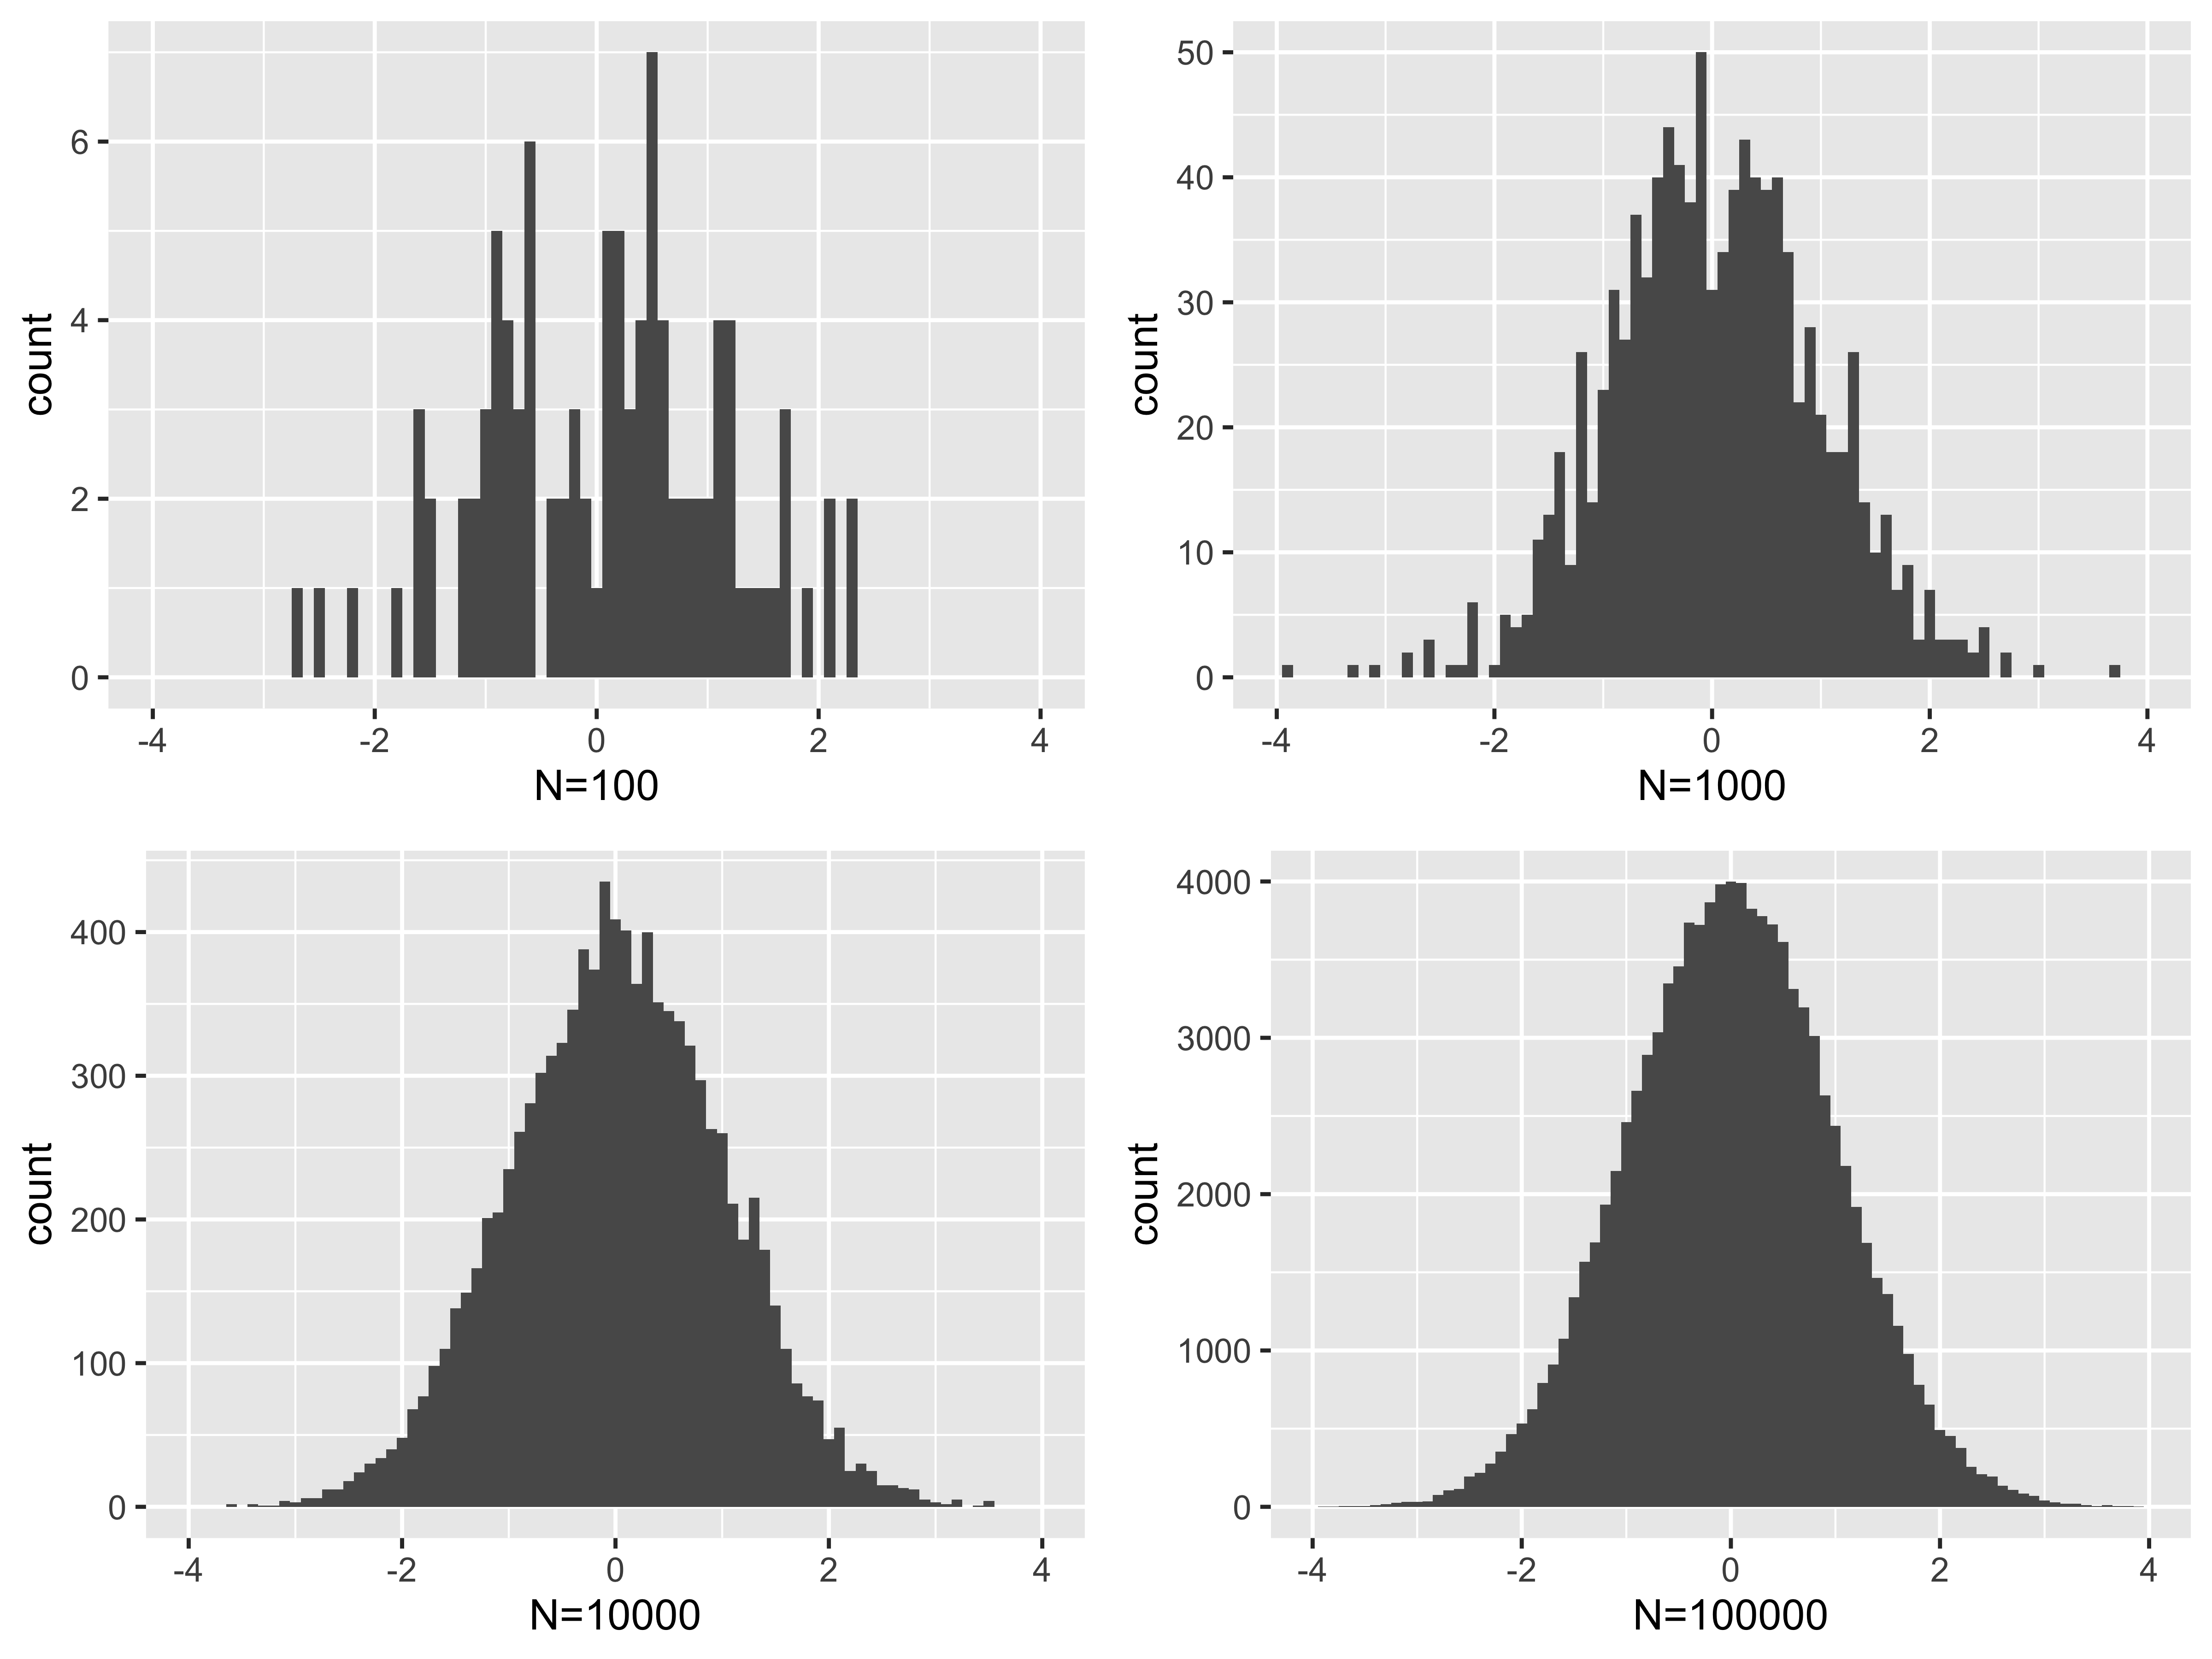
\includegraphics[keepaspectratio,width=0.8\linewidth]{../images/text25/Rplot25_01.png}
   \caption{An example of generating normal random numbers in R. As the number of samples increases, the histogram becomes almost normal distribution.}
   \label{fig::25_07}
\end{figure}


There are other advantages to using this random number generation method for approximate calculations. Instead of considering the function itself, the realized values generated from the function are stored as data, so calculating the expected value of the function can also be calculated by simply calculating the "arithmetic mean of the realized values," giving an approximate answer. With a large amount of data, calculating the descriptive statistics is the main job of statistical packages. Solving for the function's solution can be difficult due to the expansion of the equation, but statistical packages can quickly respond if given concrete examples.

In addition, statistical packages are also proficient in data processing. "Calculating the probability of getting a number of 1.0 or more for a normal distribution using integration" is a task that can be done through mathematical equations.
\[ p(x) = \int_1^{\infty} \frac{1}{\sqrt{2\pi \sigma^2}}exp\left( \frac{(x-\mu)^2}{2\sigma^2}\right) dx \]
A certain calculation is necessary (note: the confusing formula mentioned refers to the probability density function of the normal distribution, so it's not necessary to recall it. It's enough to understand that it involves integrating from 1 to infinity. If you are someone who doesn't know what an integral is, then just thinking that it's a difficult calculation should be enough.) However, if you have a random number generated from this function, selecting values greater than or equal to 1.0 from that random number and dividing it by the total number will give you an approximation of the probability - which is the relative frequency.


The difficulty in Bayesian statistics arises when dealing with functions that involve multiple interconnected parameters, since integration becomes impossible due to multiple layers of complexity. However, with the use of MCMC methods to generate random numbers from the posterior distribution, only the calculation of descriptive statistics related to the specific domain is necessary, and the complex components disappear entirely. Thanks to this technology, Bayesian statistics has recently become practical and usable.

From the next time on, I would like everyone to learn thoroughly how things change when this technology becomes "Bayesian as an estimation method". Unlike null hypothesis testing, Bayesian statistics is a recent technique and there are still few psychology papers that use it. However, as you continue to learn from now on, you will see various advantages. By the way, in Japan, only the University of Tokyo, Waseda University, and Senshu University (as of 2020) are offering psychology statistics courses focused on Bayesian statistics, and we are delivering the most advanced courses to you!

\paragraph{Appendix} Verification of Comparison between Approximation by Random Number and Theoretical Value.


I can translate the Japanese comments in the given TeX code:

\begin{lstlisting}[language=c++,label={code:25_01},caption={Approximation and Verification}]
X <- rnorm(100000,mean=0,sd=1)
length(X[X>1])/100000
# Verification
1-pnorm(1,mean=0,sd=1)
\end{lstlisting} 

The first comment reads "Approximation", which refers to the code that follows, where `rnorm` function is used to generate a random set of 100000 numbers following a normal distribution with mean 0 and standard deviation 1, stored in the variable `X`. The following line of code counts how many of these numbers are greater than 1, and then divides that value by the number of total values (100000), to get an approximation of the probability of generating a value greater than 1 from this distribution.

The second comment reads "Verification", which refers to the next line of code that calculates the true probability of generating a value greater than 1 from this distribution, using the `pnorm` function. The overall code shows an example of how to use sampling and verification to estimate probabilities of events from a given distribution.

\begin{description}
	\item[1st line] Generate 100,000 random numbers following a standard normal distribution with mean 0 and standard deviation 1, and assign them to \texttt{X}.
	\item[2nd line] Divide the length of the elements in \texttt{X} that satisfy the condition \texttt{X>1} by 100,000.
	\item[4th line] Verification based on theoretical values. Calculate the area of the corresponding section by subtracting the cumulative probability up to the probability point 1 from the total area of 1.
\end{description}


\begin{Rscreen}{Approximation by Random Numbers}{out25_01}
	\begin{verbatim}
> X <- rnorm(100000,mean=0,sd=1)
> length(X[X>1])/100000
[1] 0.15886
> 1-pnorm(1,mean=0,sd=1)
[1] 0.1586553\end{verbatim}
\end{Rscreen}

Note: There are no Japanese words in this code. The text is written in English, but the TeX code is used to format and display R code.

\section{Task}

\end{document}
